\subsubsection{Optimizing Memory Coalescing}

In this chapter, we introduce the importance of memory coalescing for effectively using memory bandwidth in CUDA.

\begin{flushleft}
    \textcolor{Green3}{\faIcon{book} \textbf{Introduction}}
\end{flushleft}
Memory bandwidth is important in CUDA because each thread may need to access memory, and efficient memory access is critical to overall performance. Ideally, when multiple threads in a CUDA program access memory, their accesses should be \emph{coalesced}. This means that \textbf{memory accesses from multiple threads are combined into a single memory transaction}.

\highspace
The memory type inside the GPU is DRAM. Since DRAM accesses are not as fast as local registers, an optimization is required. For this reason, the technique of \emph{DRAM bursts} is introduced:
\begin{itemize}
    \item It allows a block of data to be transferred in one go. When CUDA threads coalesce memory accesses, the entire burst can be used effectively, resulting in \emph{fewer memory transactions and higher memory bandwidth utilization}.

    \item By coalescing memory accesses into fewer DRAM bursts, the \emph{latency (delay) associated with memory access is reduced}. This is because once a burst is initiated, the additional data within the burst can be accessed quickly.

    \item CUDA developers use a variety of techniques to ensure that thread memory accesses are concatenated to take full advantage of DRAM burst capabilities. These include \emph{aligning data structures and managing memory access patterns}.
\end{itemize}
For \example{example}, consider a CUDA kernel where each thread accesses successive memory locations. When these accesses are combined, a single DRAM burst can fetch multiple data points needed by multiple threads, \emph{significantly speeding up the computation}.

\highspace
\begin{flushleft}
    \textcolor{Green3}{\faIcon{question-circle} \textbf{What is a DRAM burst?}}
\end{flushleft}
A \definition{DRAM (Dynamic Random Access Memory) burst} is a way of \textbf{reading data from or writing data to memory}. When accessing DRAM, \textbf{data} isn't \textbf{retrieved} one byte at a time, but rather \textbf{in bursts}. A DRAM burst involves the \textbf{transfer of multiple bytes of data in a single}, \textbf{continuous sequence}, rather than in separate, discrete chunks.

\begin{figure}[!htp]
    \centering
    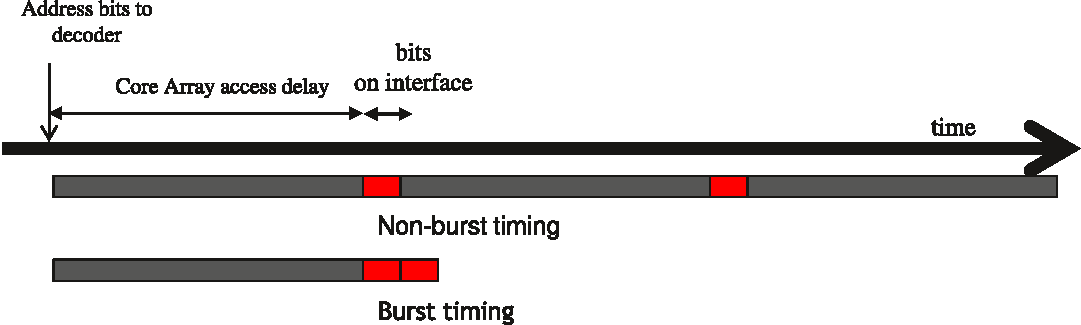
\includegraphics[width=\textwidth]{img/cuda-dram-burst-1.pdf}
    \caption{The figure shows a comparison of non-burst and burst timing in DRAM systems.}
\end{figure}
\begin{itemize}
    \item \textbf{Non-Burst Timing}. There are \textbf{gaps between data transfers}, resulting in inefficiencies.

    \item \textbf{Burst Timing}. Represents a \textbf{continuous sequence of data transfer}, illustrating the efficiency of burst mode. \textbf{Burst bytes are transmitted to the processor, but may be discarded if accesses are not sequential}.
\end{itemize}
\textbf{Burst mode minimizes the gaps between data transfers}, allowing for faster and more efficient data flow. This is in contrast to non-burst mode, where data transfers are inefficient due to gaps.

\highspace
In more detail, burst mode can be \textbf{described by the following features}:
\begin{itemize}
    \item \important{Burst operation}. \textbf{When accessing a specific memory address, the DRAM retrieves an entire block of adjacent data, called a burst}. This allows faster data access than retrieving individual bytes one at a time.
    
    \item \important{Burst Length}. The length of the burst indicates \textbf{how many bytes are transferred in one operation}. Common burst lengths are 4, 8, or 16 bytes, but larger lengths are used depending on the system and application.
    
    \item \important{Memory efficiency}. This method improves memory access efficiency. \textbf{Once the initial memory location is accessed, the DRAM can transfer the rest of the data in the burst with less overhead}.
    
    \item System Usage. Burst transfers are particularly useful in applications where large blocks of data must be moved quickly, such as graphics processing where textures and images are frequently accessed.
\end{itemize}

\begin{examplebox}[: great analogy with burst technology]
    We can think of burst mode as a bookshelf, where instead of taking out one book at a time, we take out a whole section at once. This way, we get more books (data) in one go, reducing the time it takes to reach for each book individually.
\end{examplebox}

\newpage

\noindent
The following figure shows a system view of the DRAM burst. Each address space is divided into burst sections, and when one location is accessed, all other locations in the same section are also delivered to the processor.

\begin{figure}[!htp]
    \centering
    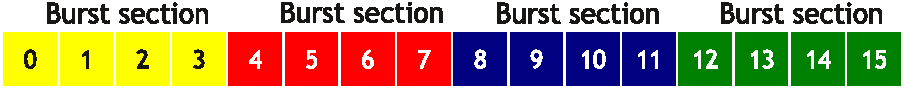
\includegraphics[width=.8\textwidth]{img/cuda-dram-burst-2.pdf}
    \caption{In the figure, a 16-byte address space is divided into 4-byte burst sections. In practice, address spaces are much larger (e.g., 4 GB) and burst sections are also larger (e.g., 128 bytes or more).}
\end{figure}

\noindent
\begin{flushleft}
    \textcolor{Green3}{\faIcon{balance-scale} \textbf{Coalesced access vs un-coalesced access}}
\end{flushleft}
\definition{Memory Coalescing} refers to the \textbf{process of combining} (or \emph{coalescing}) \textbf{multiple memory accesses by different threads into a single memory transaction}. This is important in the context of GPUs because they run many threads in parallel, and efficient memory access can significantly improve performance.

\highspace
\textbf{When threads in a warp} (a group of threads running in parallel) \textbf{access successive memory locations, these accesses are combined into a single memory transaction}. This means that all requested data is retrieved in one go.

\highspace
When threads access memory locations that are scattered or misaligned, multiple memory transactions are required, leading to inefficiencies. This phenomenon is called \definition{Un-Coalesced Access}.

\highspace
\textbf{Un-Coalesced Accesses} occur when the \textbf{memory requests of multiple threads in a warp do not fit properly into a single memory transaction}. This inefficiency results in \emph{increased memory latency} and \emph{lower overall performance}. It is manifested when:
\begin{itemize}
    \item \important{Non-Sequential Memory Access}. When threads access memory addresses that are not contiguous, the \textbf{memory controller must handle each access individually or in smaller, less efficient chunks}.
    
    \item \important{Crossing Burst Boundaries}. When memory accesses span multiple DRAM burst sections, \textbf{multiple memory transactions are required}. Each burst section may only be able to handle a portion of the requested data, resulting in additional overhead.

    \item \important{Thread misalignment}. If the \textbf{data being accessed by threads is misaligned with the natural boundaries of memory bursts}, the accesses cannot be merged effectively. This often happens with poorly structured data layouts.
\end{itemize}
The un-coalesced accesses are a \textbf{penalty for memory optimization because the memory controller cannot combine these accesses into a single transaction because they are spread out}. Instead, it must handle multiple transactions, each fetching only a few bytes relevant to the threads.

\highspace
The \textbf{consequences of un-coalesced access} are:
\begin{itemize}
    \item \important{Increased DRAM transactions}. \textbf{Each un-coalesced access requires a separate DRAM burst}, increasing the number of memory transactions.

    \item \important{Wasted Bandwidth}. \textbf{Not all bytes in a DRAM burst are utilized}. For example, if each burst fetches 32 bytes and only 8 bytes are used by threads, the remaining 24 bytes are wasted.

    \item \important{Higher Latency}. More transactions means more latency because \textbf{each transaction requires setup and transmission time}.
\end{itemize}

\begin{figure}[!htp]
    \centering
    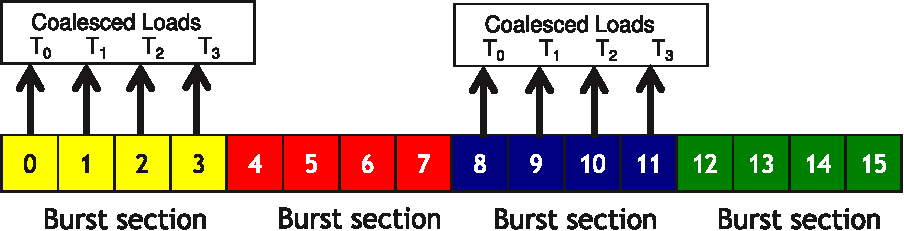
\includegraphics[width=.8\textwidth]{img/cuda-memory-coalescing-1.pdf}
    \caption{When all threads of a warp execute a load instruction, if all accessed locations are in the same burst section, only one DRAM request is made and the access is fully merged.}
\end{figure}

\begin{figure}[!htp]
    \centering
    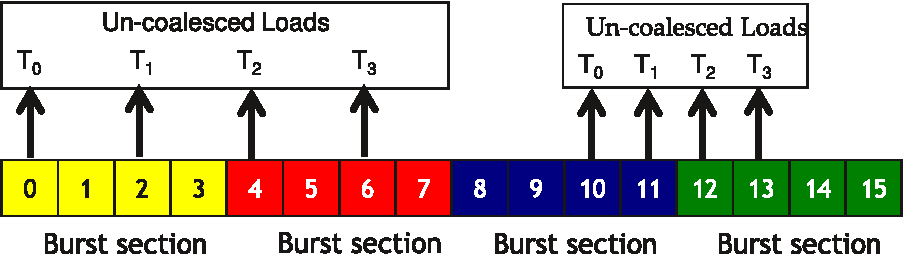
\includegraphics[width=.8\textwidth]{img/cuda-memory-un-coalesced-1.pdf}
    \caption{If the accessed locations are spread across burst boundaries, coalescing fails (un-coalesced accesses), multiple DRAM requests are made. This results in some garbage bytes that are not used by threads.}
\end{figure}

\begin{examplebox}[: great analogy to un-coalesced access]
    Think of un-coalesced access as trying to get multiple items from different aisles in a supermarket, one at a time. We end up walking back and forth more and taking longer to collect all the items than if we collected items from a single, well-organized aisle.
\end{examplebox}

\newpage

\begin{examplebox}[: difference from coalesced and un-coalesced access]
    Suppose a warp of 32 threads accesses an array in global memory. If each thread accesses elements sequentially (thread 0 accesses element 0, thread 1 accesses element 1, and so on), \textbf{a single memory transaction retrieves all 32 elements}.

    In contrast, if the same warp accesses memory in a non-sequential manner (thread 0 accesses element 0, thread 1 accesses element 4, thread 2 accesses element 8, and so on), \textbf{multiple memory transactions are required}, reducing efficiency.
\end{examplebox}
